\documentclass[12pt]{article}
\usepackage[export]{adjustbox}
\usepackage{amsfonts, amsmath, amssymb}
\usepackage{appendix}
\usepackage{bm}
\usepackage{chemformula}
\usepackage{csquotes}
\usepackage[es]{datetime2}
\usepackage{enumitem}
\usepackage{empheq}
\usepackage{fancyhdr}
\usepackage{fontspec}
\usepackage{geometry}
\usepackage{graphicx}
\usepackage{kantlipsum}
\usepackage{lastpage}
\usepackage{linebreaker} % line-breaker algorithm in LuaLaTeX
\usepackage{lualatex-math} % Fixes for mathematics
\usepackage{mathtools}
\usepackage{microtype}
\usepackage{mismath}
\usepackage{siunitx}
\usepackage{subcaption}
\usepackage{tabularray}
\usepackage{titling}
\usepackage{xcolor}
\usepackage{xspace}
\usepackage{polyglossia}
\usepackage[
    sorting = none
]{biblatex}
\usepackage{hyperref}
\setmainlanguage{spanish}
% \setmainlanguage[variant=mexican]{spanish}
\usepackage{cleveref}
\gappto\captionsspanish{\renewcommand{\tablename}{Tabla}} % Table's caption name
\crefname{table}{Tabla}{Tablas} % Table's cross-reference name
\crefname{figure}{Fig.}{Figs.} % Figure's cross-reference name
\crefname{equation}{}{} % Equation's cross-reference name

\setlength{\parindent}{2em} % Sangría
\setlength{\parskip}{0.5em} % Espacio entre párrafos
\linespread{1.1} % line spacing
\setlength{\jot}{10pt} % Space between lines in multiline eqs

\newcommand{\idest}{\emph{i.e.},\xspace} % id est
\DTMsavedate{duedate}{2023-05-23}

\geometry{
    letterpaper,
    margin = 0.6in,
    includefoot
}

% Line-breaker config
\linebreakersetup {
    maxtolerance = 90,
    maxemergencystretch = 1em,
    maxcycles = 4
}

\graphicspath{{./img/}{./img/plots/}}

\hypersetup{
    colorlinks = true,%
    linkcolor={[rgb]{0,0.2,0.6}},%
    citecolor={[rgb]{0,0.6,0.2}},%
    filecolor={[rgb]{0.8,0,0.8}},%
    urlcolor={[rgb]{0.8,0,0.8}},%
    runcolor={[rgb]{0.8,0,0.8}},% 
    menucolor={[rgb]{0,0.2,0.6}},%
    linkbordercolor={[rgb]{0,0.2,0.6}},%
    citebordercolor={[rgb]{0,0.6,0.2}},%
    filebordercolor={[rgb]{0.8,0,0.8}},%
    urlbordercolor={[rgb]{0.8,0,0.8}},%
    runbordercolor={[rgb]{0.8,0,0.8}},%
    menubordercolor={[rgb]{0,0.2,0.6}},% 
    pdftitle={Práctica 3: Detectores centelladores con fotomultiplicadores},%
    pdfauthor={López Merino Marcos, Abraham Jain Jiménez},%
    pdfsubject={Introducción a la Física Nuclear},%
    pdfkeywords={Facultad de Ciencias, UNAM, Introducción a la Física Nuclear, Experimental},%
    unicode = true%
}

\sisetup{
	output-decimal-marker = {.}, 
	per-mode = symbol-or-fraction,
	separate-uncertainty = true,
	exponent-product = \mul,
    inter-unit-product = \ensuremath{{}\cdot{}}
}


\definecolor{base3}{RGB}{253, 246, 227}%
\definecolor{pinkwave}{RGB}{255, 0, 128}%
\definecolor{FCBlue}{RGB}{11, 61, 98}%
\pagecolor{base3}

\setlength{\droptitle}{-60pt} % raise the title
\pretitle{\begin{center}\large\bfseries}
\newcommand{\subtitle}[1]{%
  \posttitle{%
    \par\LARGE #1
    \end{center}
    \vskip 0.25em
    }%
}
\preauthor{\begin{center}
\large \lineskip 0.5em%
\begin{tabular}[t]{c}}
\postauthor{\end{tabular}\par\end{center}}
\predate{\begin{center}\small\bfseries}
\postdate{\end{center}}


\title{Práctica 3}
\subtitle{Detectores centelladores con fotomultiplicadores}
\author{%
    Abraham Jain Jiménez \\ \href{mailto:jain@ciencias.unam.mx}{\footnotesize jain@ciencias.unam.mx}
  \and Marcos López Merino \\ \href{mailto:marcoslm@ciencias.unam.mx}{\footnotesize marcoslm@ciencias.unam.mx}
}%
\date{Entrega: \DTMusedate{duedate}}

% Encabezado y pie de página
\setlength{\headheight}{43pt}
\renewcommand{\headruleskip}{5pt}

\pagestyle{fancy}
\lhead{\parbox{0.33\textwidth}{Introducción a la Física Nuclear Grupo 8316}}
\chead{}
\rhead{
\includegraphics[scale = 0.25, valign = c]{LogoFCUNAMcolor.pdf}}
\renewcommand{\headrule}{
    \begin{minipage}{\textwidth}%
        \color{FCBlue} \hrule width \hsize height 2pt \kern 1mm \hrule width \hsize
    \end{minipage}
}

\lfoot{}
\cfoot{}
\rfoot{Pág. \thepage \hspace{1pt} de \pageref{LastPage}}
\renewcommand{\footrule}{
    \begin{minipage}{1\textwidth}%
        \color{FCBlue} \hrule width \hsize height 0.5pt  
    \end{minipage}\par
    
}%

\addbibresource{bibliography.bib}

\begin{document}
    \maketitle
    \thispagestyle{fancy}
    \begin{abstract}
        \kant[1]
    \end{abstract}

    \section*{Introducción}
        El montaje del sistema con el que nos corresponde trabajar consitió de dos fuentes radiactivas de decaimiento tipo beta (\ch{^{60} Co} y \ch{^{137} Cs}), dos cristales centelladores inorgánicos (\ch{CsI (Tl)} y \ch{BGO (Bi Ge O)}), fuente de voltaje (TENNELEC TC 952), amplificador modelo 572\cite{Amplifier572}, ADC\cite{USC30ADC} y una computadora. El montaje se muestra en la \cref{fig:montaje}.

        \begin{figure}[htb]
            \centering
            \includegraphics{example-image-a}
            \caption{Diagrama del montaje experimental para la detección de partículas.}
            \label{fig:montaje}
        \end{figure}

        Existen diferentes tipos de detectores, cada uno con características propias que los hacen más o menos adecuados para la detección de cierto tipo de partículas. En esta práctica se trabajó con detectores centelladores inórganicos.

        Un centellador 
    
    \section*{Desarrollo experimental}
        \subsection*{Calibración de energía}
        Una de las tareas principales de cualquier análisisen un experimento en el campo de la física nuclear experimental a bajas energías es la calibración de la energía, \idest necesitamos encontrar una relación entre los canales \(\text{Ch}\) en el centro del fotopico y la energía correspondiente a cada una de las gammas \(E_{\gamma}\). Esta relación tiene la forma

        \begin{equation}
            E_{\gamma}(\text{Ch}) = m \cdot \text{Ch} + b,
            \label{eq:linear_model}
        \end{equation}

        donde \(m\) es la pendiente y \(b\) es la intersección de la energía cuando \(\text{Ch} = 0\).

        En esta práctica se utilizaron dos centelladores diferentes: \ch{CsI (Tl)} y \ch{BGO (BiGeO)}, por lo que se obtuvieron dos relaciones diferentes. Además, se hizo uso de la función \texttt{Peak Finder} del software USX\cite{usxSoftware} para encontrar el centroide de cada uno de los fotopicos.

        \subsubsection*{Calibración para el centellador \ch{CsI (Tl)}}

        Para la calibración del centellador \ch{CsI (Tl)} el valor correspondiente a la energía de las gammas de \ch{^{137} Cs} y \ch{^{60} Co} se obtuvo de la base de datos del \emph{National Nuclear Data Center}\cite{ENSDF}. Los datos obtenidos se muestran en la \cref{tab:csiCalibration}.

        \begin{table}[htb]
            \centering
            \begin{tblr}{
                colspec = {cc},
                hlines,
                rowsep = 4pt,
                row{1} = {font = \bfseries}
            }
                Channel & {Energía \\ (\si{\keV})}  \\
                404     & 661.657 \\             
                725     & 1173.228 \\
                825     & 1332.492
            \end{tblr}
            \caption{Datos de la energía de las gammas de \ch{^{137} Cs} y \ch{^{60} Co} con el centroide de los fotopicos para la calibración del centellador \ch{CsI (Tl)}.}
            \label{tab:csiCalibration}
        \end{table}

        La relación entre la energía y el canal para el centellador \ch{CsI (Tl)} que se obtuvo se muestra en la \cref{fig:csiCalibration} y tiene la forma

        \begin{equation}
            E_{\gamma}(\text{Ch}) = \qty{1.5937 \pm 0.002509}{\keV} \cdot \text{Ch} + \qty{17.7236 \pm 0.1695}{\keV}.
            \label{eq:csiCalibration}
        \end{equation}

        \begin{figure}[!htb]
            \centering
            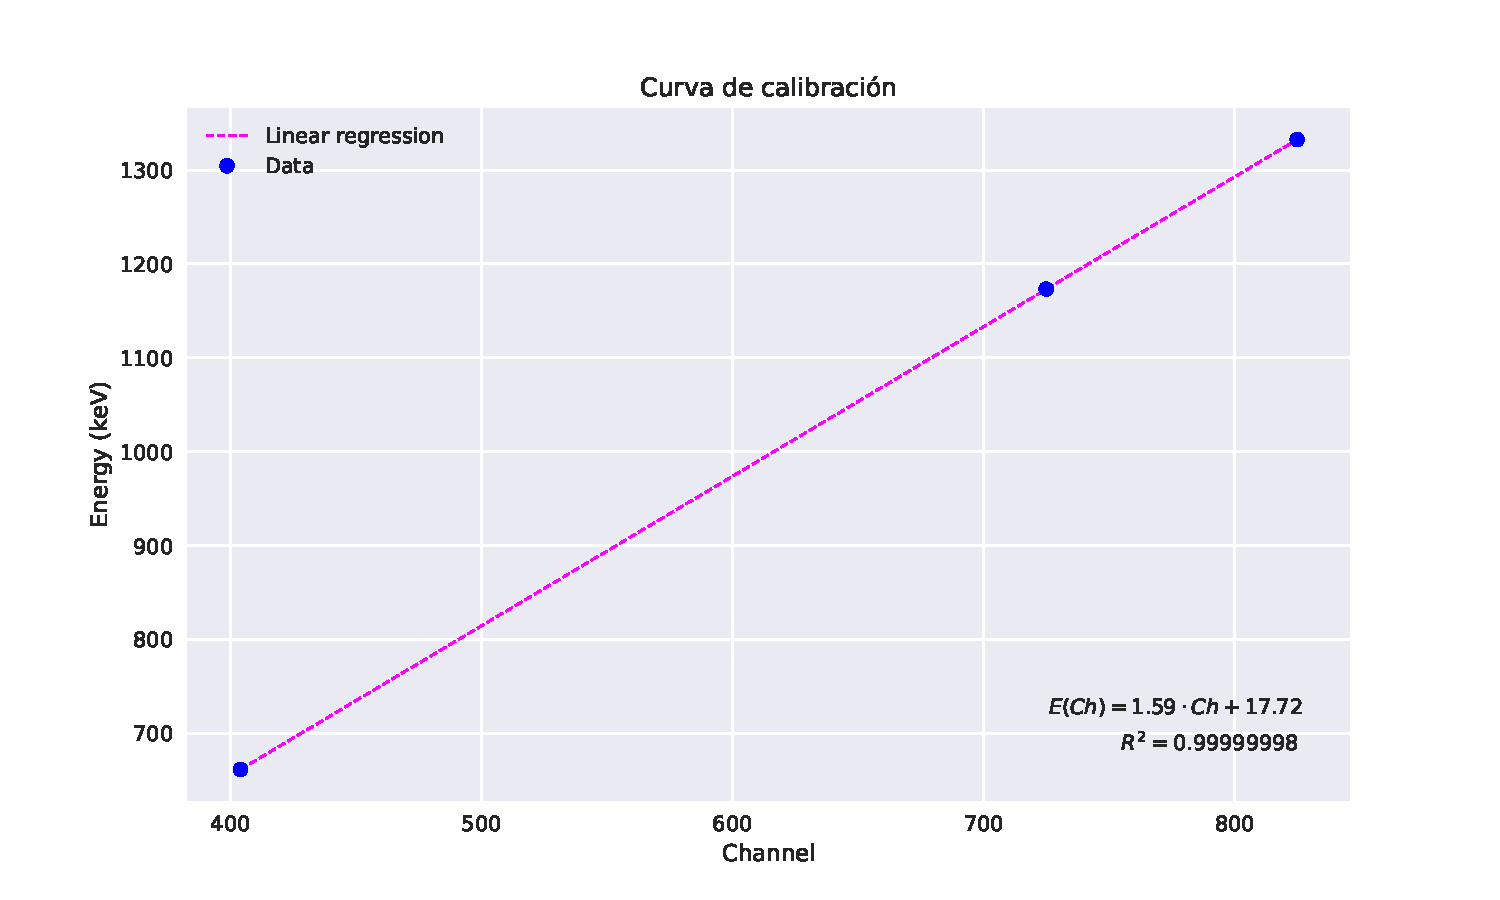
\includegraphics[scale = 0.7]{csi_calibration.pdf}
            \caption{Recta de calibración de energía para el centellador \ch{CsI (Tl)}.}
            \label{fig:csiCalibration}
        \end{figure}

        \subsubsection*{Calibración para el centellador \ch{BGO (BiGeO)}}

        La calibración del centellador \ch{BGO (BiGeO)} se realizó de forma similar a la del centellador \ch{CsI (Tl)} y los datos obtenidos se muestran en la \cref{tab:bgoCalibration}.

        \begin{table}[htb]
            \centering
            \begin{tblr}{
                colspec = {cc},
                hlines,
                rowsep = 4pt,
                row{1} = {font = \bfseries}
            }
                Channel & {Energía \\ (\si{\keV})}  \\
                272     & 661.657 \\             
                502     & 1173.228 \\
                572     & 1332.492
            \end{tblr}
            \caption{Datos de la energía de las gammas de \ch{^{137} Cs} y \ch{^{60} Co} con el centroide de los fotopicos para la calibración del centellador \ch{BGO (BiGeO)}.}
            \label{tab:bgoCalibration}
        \end{table}

        La relación entre la energía y el canal para el centellador \ch{BGO (BiGeO)} que se obtuvo se muestra en la \cref{fig:bgoCalibration} y tiene la forma

        \begin{equation}
            E_{\gamma}(\text{Ch}) = \qty{2.2332 \pm 0.009618}{\keV} \cdot \text{Ch} + \qty{53.8501 \pm 4.4880}{\keV}.
            \label{eq:bgoCalibration}
        \end{equation}

        \begin{figure}[!htb]
            \centering
            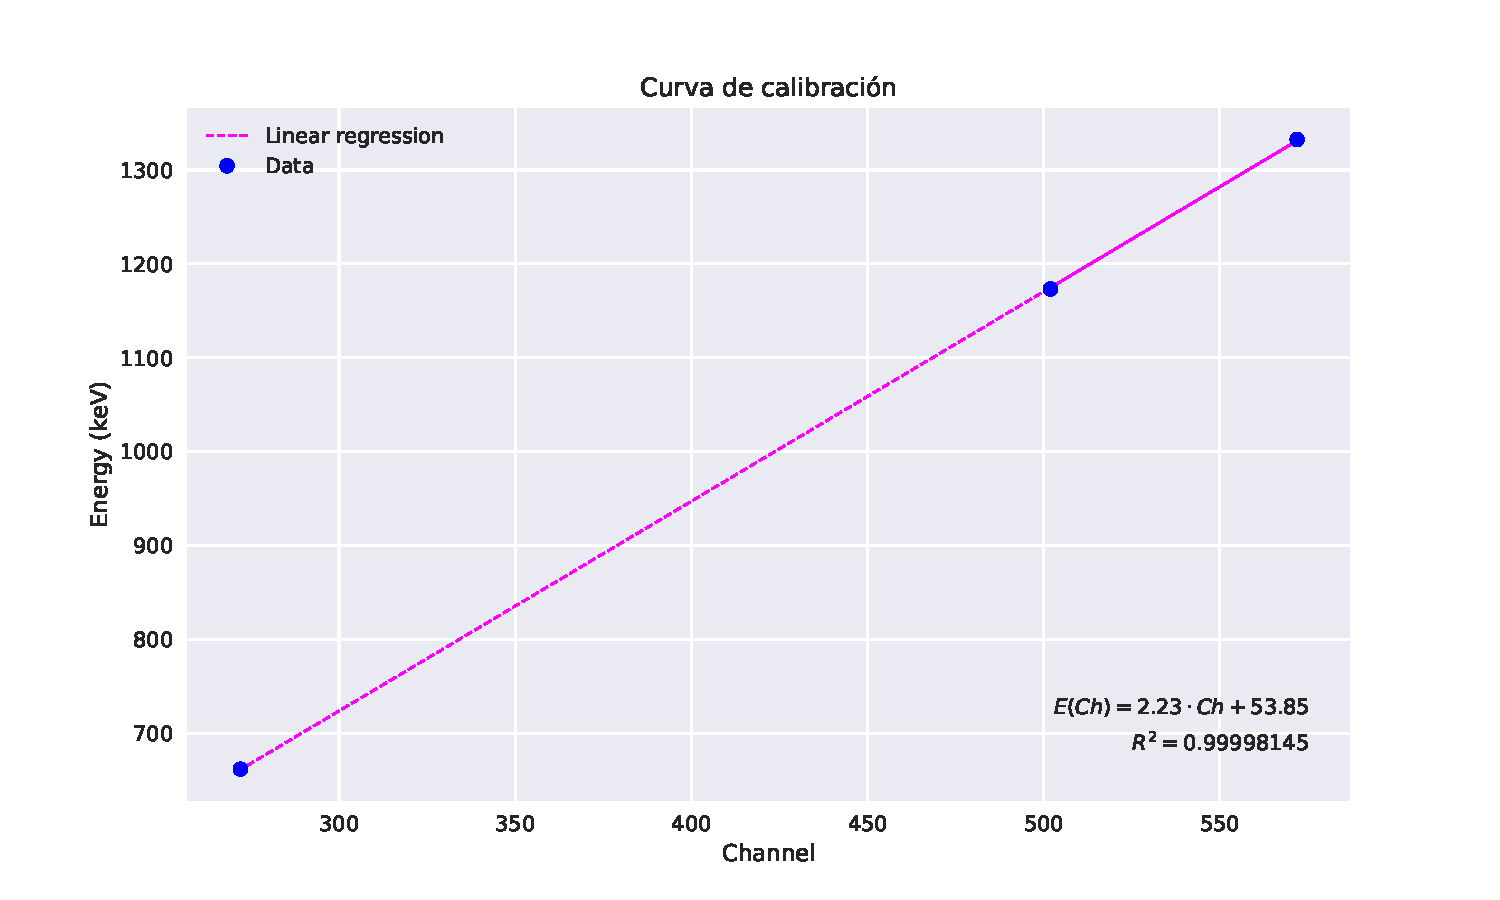
\includegraphics[scale = 0.7]{bgo_calibration.pdf}
            \caption{Recta de calibración de energía para el centellador \ch{BGO (BiGeO)}.}
            \label{fig:bgoCalibration}
        \end{figure}

    \subsection*{Espectros de energía}

    A partir de las \cref{eq:csiCalibration,eq:bgoCalibration} se obtuvieron los espectros de Energía contra Número de cuentas para cada uno de los centelladores. Estos espectros se muestran en las \cref{fig:csiCoSpectrum,fig:bgoCsSpectrum}.

    \subsubsection*{Espectro de energía para el centellador \ch{CsI (Tl)}}

    \begin{figure}[!htb]
        \centering
        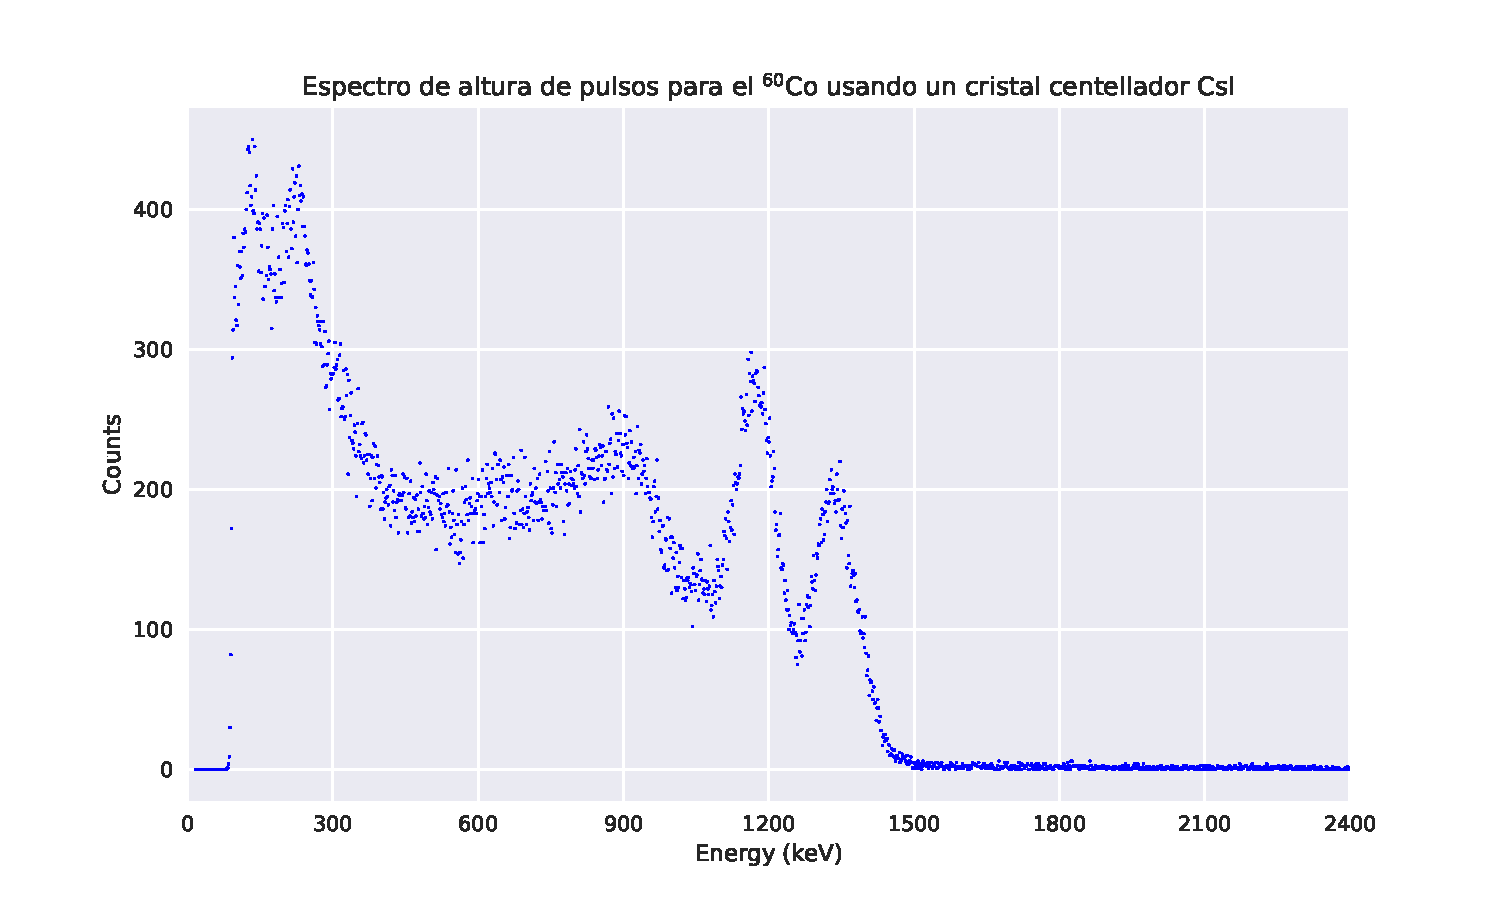
\includegraphics[scale = 0.7]{energy_spectrum_CsICo.pdf}
        \caption{Espectro de energía para el centellador \ch{CsI (Tl)} con la fuente de \ch{^{60} Co}.}
        \label{fig:csiCoSpectrum}
    \end{figure}

    \begin{figure}[!htb]
        \centering
        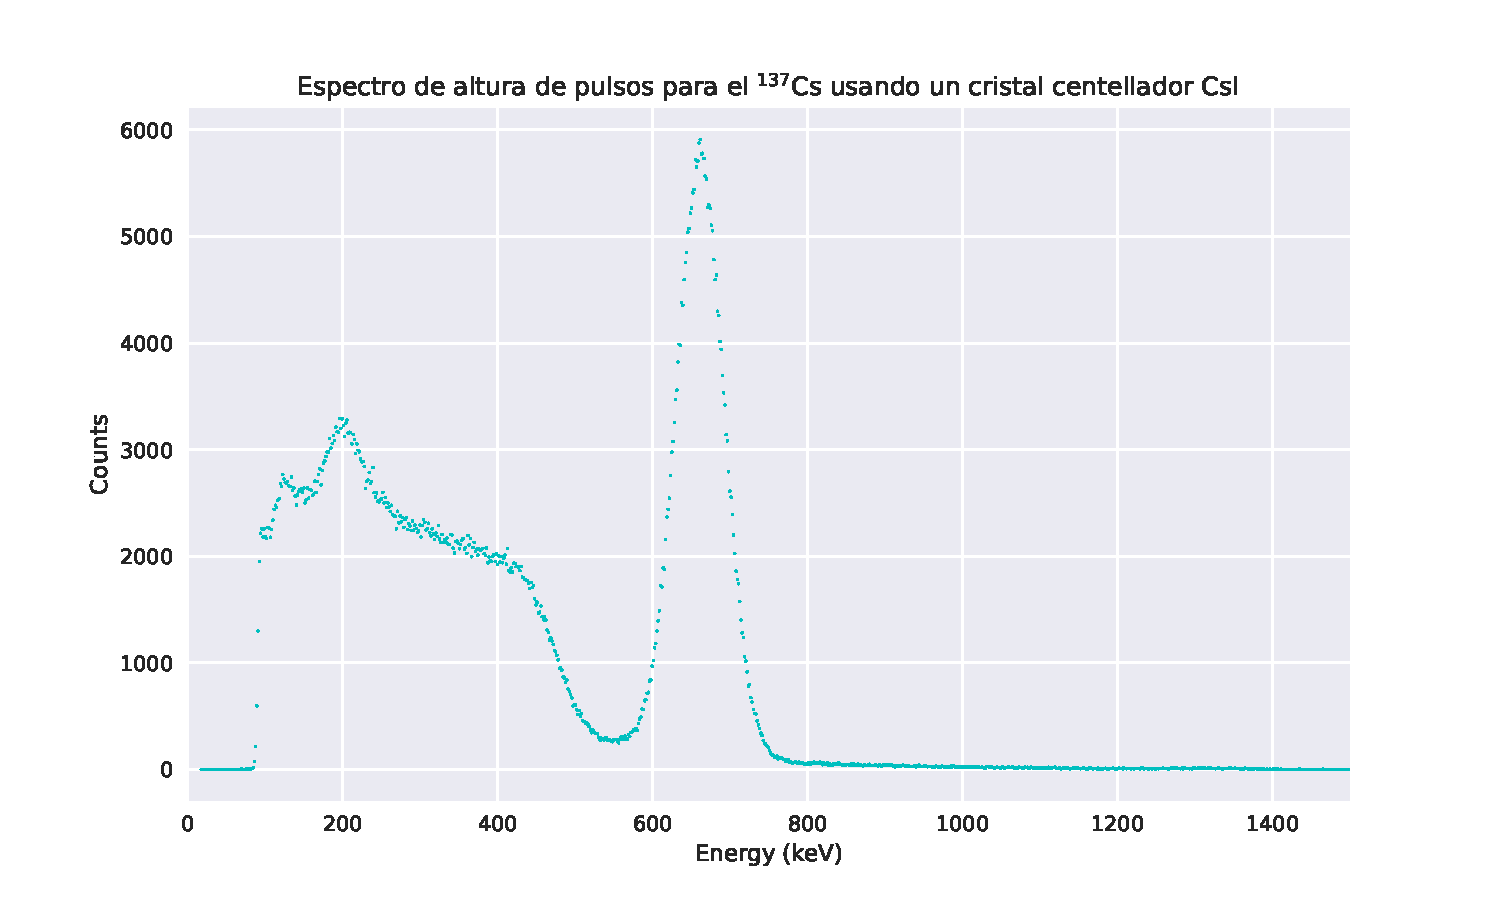
\includegraphics[scale = 0.7]{energy_spectrum_CsICs.pdf}
        \caption{Espectro de energía para el centellador \ch{CsI (Tl)} con la fuente de \ch{^{137} Cs}.}
        \label{fig:csiCsSpectrum}
    \end{figure}

    \subsubsection*{Espectro de energía para el centellador \ch{BGO (BiGeO)}}

    \begin{figure}[!htb]
        \centering
        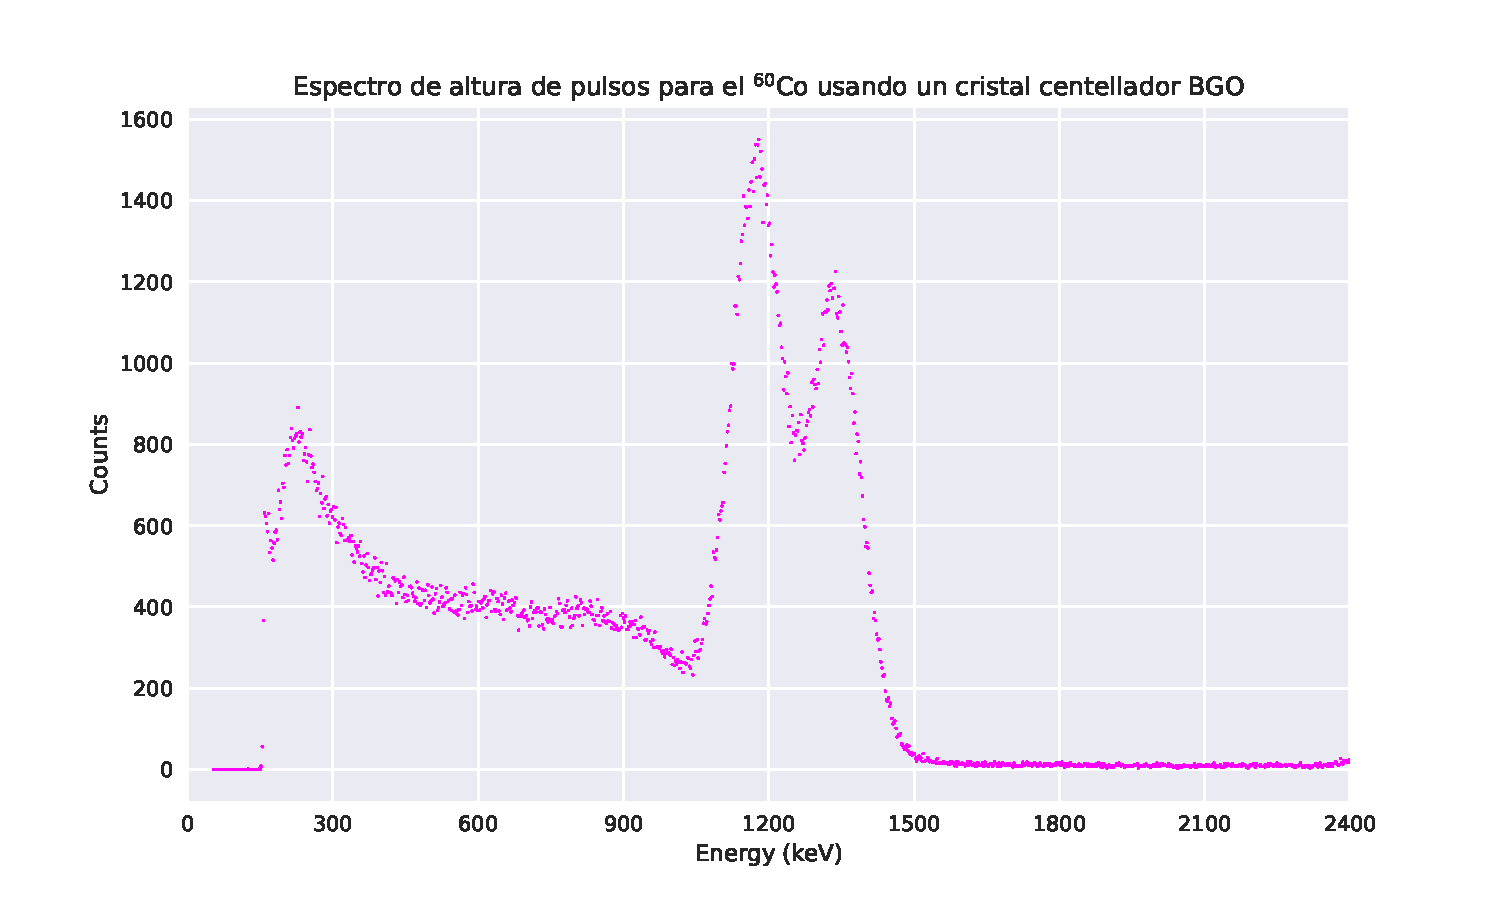
\includegraphics[scale = 0.7]{energy_spectrum_BGOCo.pdf}
        \caption{Espectro de energía para el centellador \ch{BGO (BiGeO)} con la fuente de \ch{^{60} Co}.}
        \label{fig:bgoCoSpectrum}
    \end{figure}

    \begin{figure}[!htb]
        \centering
        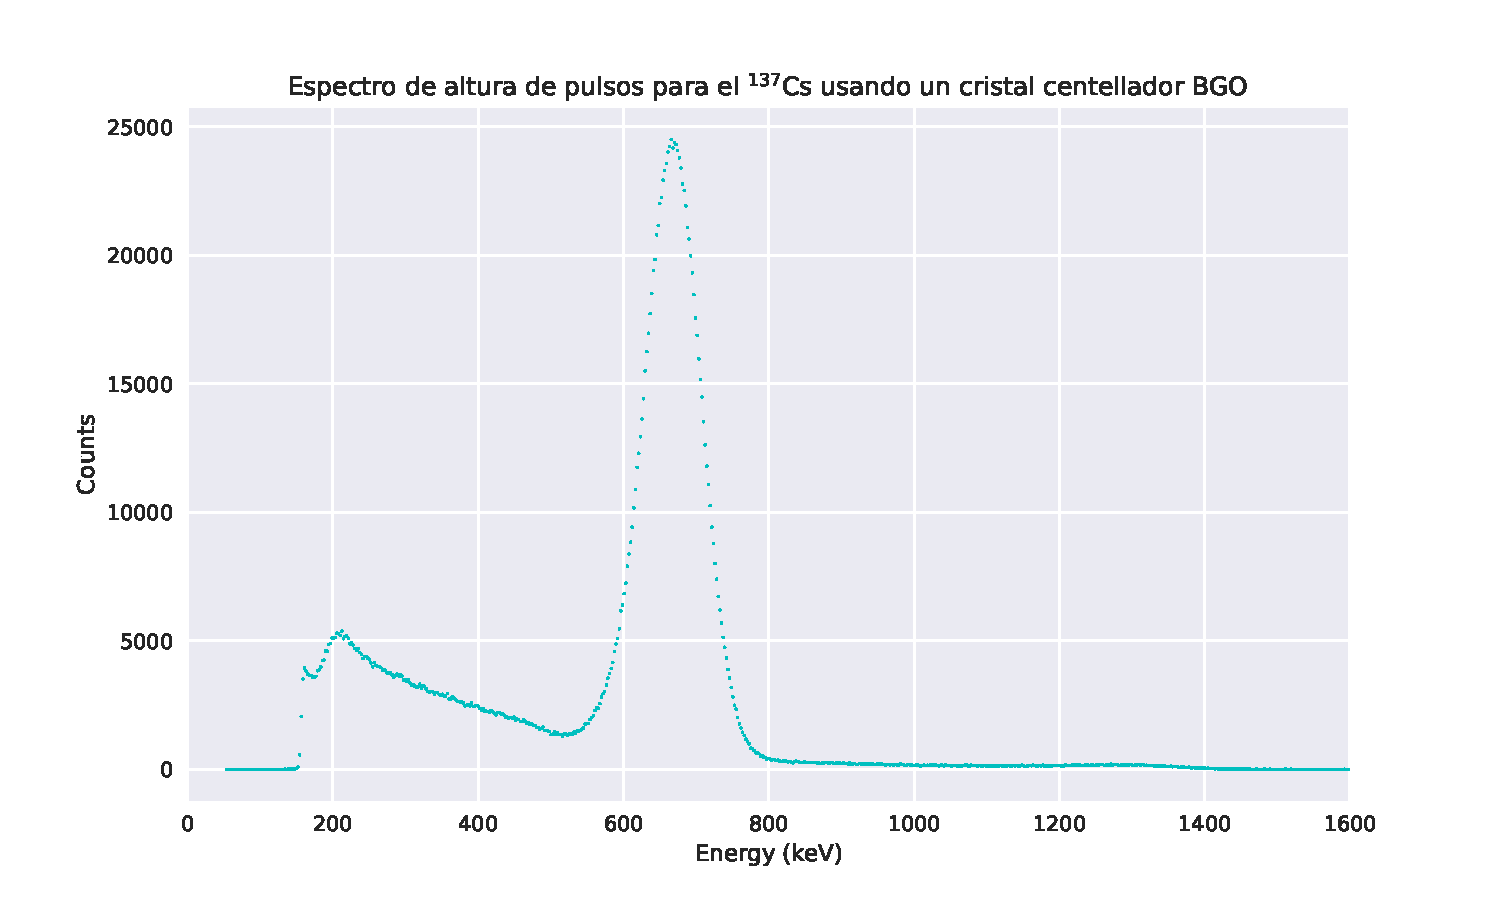
\includegraphics[scale = 0.7]{energy_spectrum_BGOCs.pdf}
        \caption{Espectro de energía para el centellador \ch{BGO (BiGeO)} con la fuente de \ch{^{137} Cs}.}
        \label{fig:bgoCsSpectrum}
    \end{figure}

    \section*{Discusión}
    
    Recordemos que el ancho del fotopico es una medida de la resolución del sistema de detección. La resolución habitualmente es definida como el cociente entre el \(\text{FWHM}\) del fotopico y \(E_{0}\) que es la energía correspondiente a las gammas, \idest el centroide de la distribución.

    \begin{equation}
        R = \dfrac{\text{FWHM}}{E_{0}} \cdot \qty{100}{\percent},
        \label{eq:resolution}
    \end{equation}

    donde \(\text{FWHM} = 2.35\sigma\).
    
    \subsection*{Resolución del centellador \ch{CsI (Tl)}}

    A partir de \cref{eq:resolution} calculamos la resolución para cada uno de los fotopicos, tal que

    \begin{align*}
        R_{\ch{Co}1} &= \qty{0.2266}{\percent}, \\
        R_{\ch{Co}2} &= \qty{0.1408}{\percent}, \\
        R_{\ch{Cs}} &= \qty{0.0537}{\percent}.
    \end{align*}

    Notamos que la resolución es mejor para el fotopico de \ch{^{137} Cs} que para los fotopicos de \ch{^{60} Co}. Esto se debe a que la energía de las gammas de \ch{^{137} Cs} es menor que la energía de las gammas de \ch{^{60} Co} y por lo tanto la resolución es mejor.

    Por lo que la resolución de nuestras mediciones es

    \begin{equation*}
        R = \qty{0.0537}{\percent}.
    \end{equation*}

    \subsection*{Resolución del centellador \ch{BGO (BiGeO)}}

    La resolución para cada uno de los fotopicos usando el centellador \ch{BGO (BiGeO)} se muestra a continuación

    \begin{align*}
        R_{\ch{Co}1} &= \qty{0.1239}{\percent}, \\
        R_{\ch{Co}2} &= \qty{0.0769}{\percent}, \\
        R_{\ch{Cs}} &= \qty{0.0293}{\percent}.
    \end{align*}

    Para este caso, sucede lo mismo que para el centellador \ch{CsI (Tl)}, la resolución es mejor para el fotopico de \ch{^{137} Cs} que para los fotopicos de \ch{^{60} Co}. Por lo que la resolución de nuestras mediciones es

    \begin{equation*}
        R = \qty{0.0293}{\percent}.
    \end{equation*}

    \subsection*{Hombro Compton}

    Otra forma en la que interactúan los rayos gamma con el cristal centellador es por medio de la dispersión de Compton. La dispersión de Compton es una dispersión puramente cinemática de un fotón incidente de energía \(E_{\gamma}\) con un electrón en el cristal centellador.

    Notemos que en el espectro Compton (ver \cref{fig:comptonSpectrum}) el pico de deflección (\emph{backscatter peak}) a bajos voltajes ocurre cuando los fotones golpean el detector y son dispersados hasta el centellador con una energía menor. La parte más plana del espectro (\emph{Compton plateau}) ocurre cuando los fotones son dispersados en el centellador. Es decir, la energía del electrón deflectado es detectada, mientras que los fotones pasan desapercibidos. La energía varía de un máximo en el Hombro Compton, cuando los fotones son deflectados con un ángulo de \qty{180}{\degree}, a cero cuando los fotones son dispersados con un ángulo de \qty{0}{\degree}.

    \begin{figure}[!htb]
        \centering
        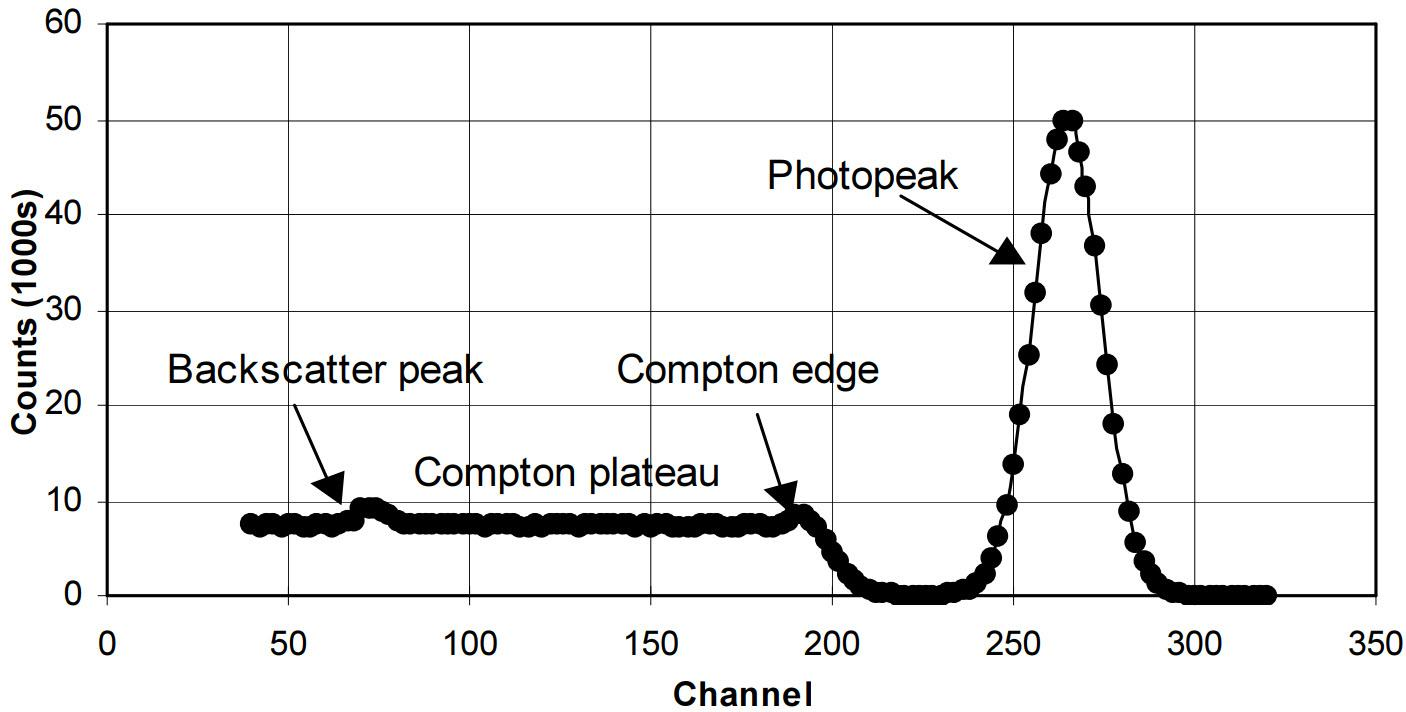
\includegraphics{compton_spectrum.jpg}
        \caption{Ejemplo de un espectro de altura para una fuente de rayos gammas en el que están presentes la dispersión de Compton y el efecto fotoeléctrico.\cite{gammaSpectroscopy}}
        \label{fig:comptonSpectrum}
    \end{figure}

    Ocasionalmente, un rayo gamma dispersado en el centellador puede intereactuar via el efecto fotoeléctrico. De esta manera, debemos calcular la energía para este caso, a través de

    \begin{equation}
        \Delta E_{C} = \dfrac{E}{1 + \dfrac{2E}{m_{\e}c^{2}}},
        \label{eq:comptonEnergy}
    \end{equation}

    donde \(E\) es la energía de la gamma y \(m_{\e}c^{2}\) la energía en reposo del electrón en \unit{\keV}. Mientras que la energía máxima, el Hombro Compton, se obtiene mediante

    \begin{equation}
        E_{HC} = E - \Delta E_{C}.
        \label{eq:comptonEdge}
    \end{equation}

    Es necesario mencionar que si el espectro tiene más de un fotopico, cada uno de estos picos tendrá un Hombro Compton asociado.

    \subsubsection*{Hombro Compton usando el centellador \ch{CsI (Tl)}}

    A partir de \cref{eq:comptonEnergy,eq:comptonEdge} tenemos que el Hombro Compton para cada una de las fuentes radioactivas es

    \begin{align*}
        E_{HC}^{\ch{^{60} Co}} &= \qty{963.42}{\keV},\\
        E_{HC}^{\ch{^{137} Cs}} &= \qty{477.25}{\keV}.
    \end{align*}

    Estos valores se encuentran representados aproximadamente mediante círculos en las \cref{fig:comptonEdgeCsICo,fig:comptonEdgeCsICs}.

    \begin{figure}[!htb]
        \centering
        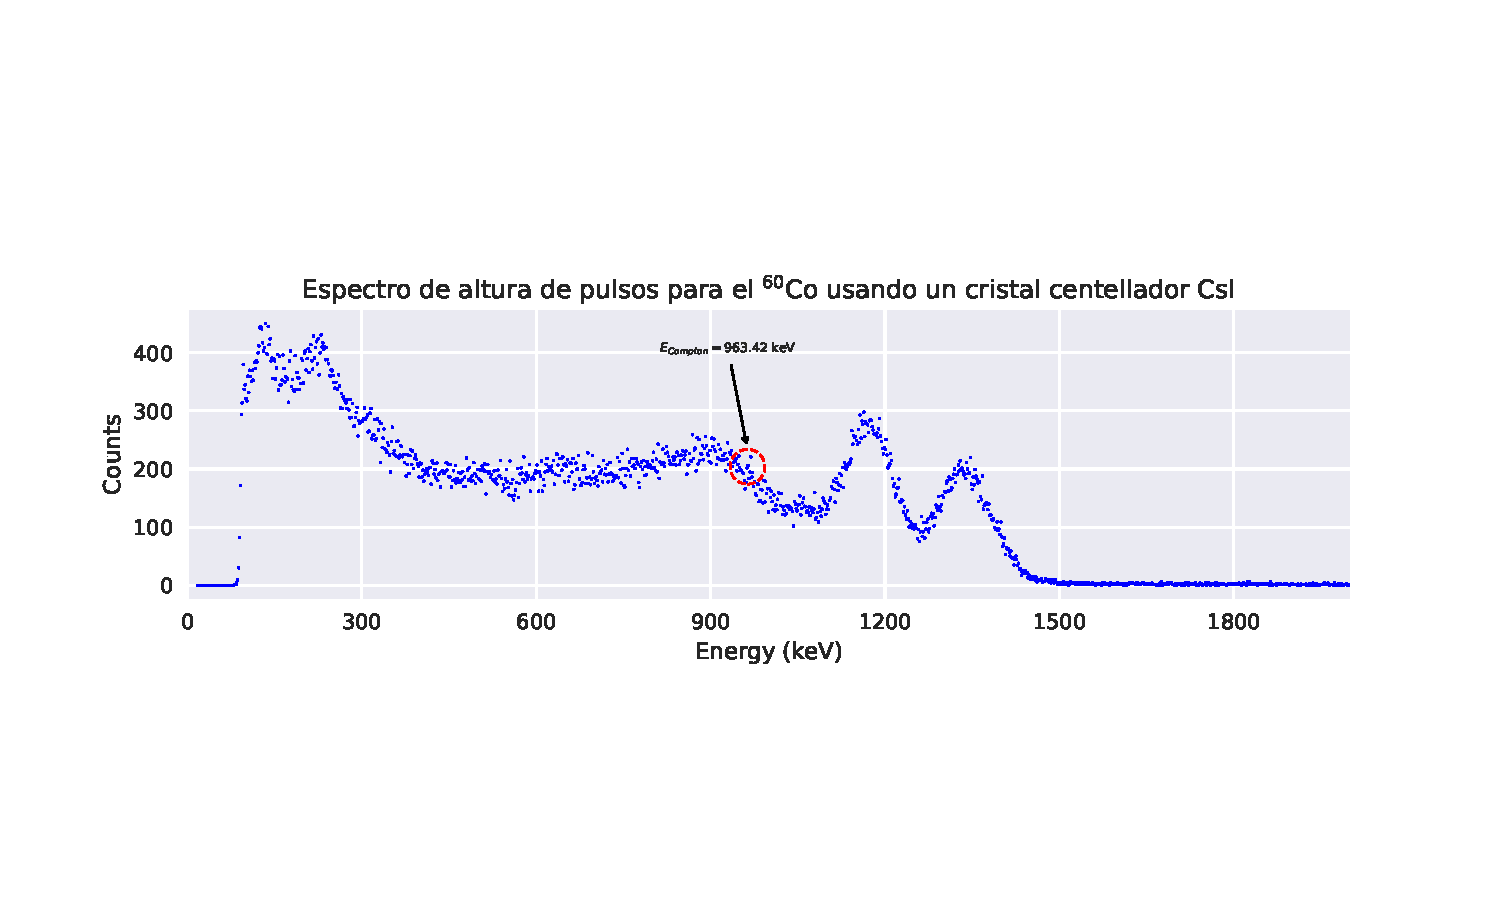
\includegraphics[trim={1cm 3.75cm 1cm 3.75cm}, width=\textwidth, clip]{compton_edge_CsICo.pdf}
        \caption{Espectro de energía contra número de cuentas para la fuente de \ch{^{60} Co} usando el centellador \ch{CsI (Tl)}. El valor del Hombro Compton está representado por el círculo.}
        \label{fig:comptonEdgeCsICo}
    \end{figure}

    \begin{figure}[!htb]
        \centering
        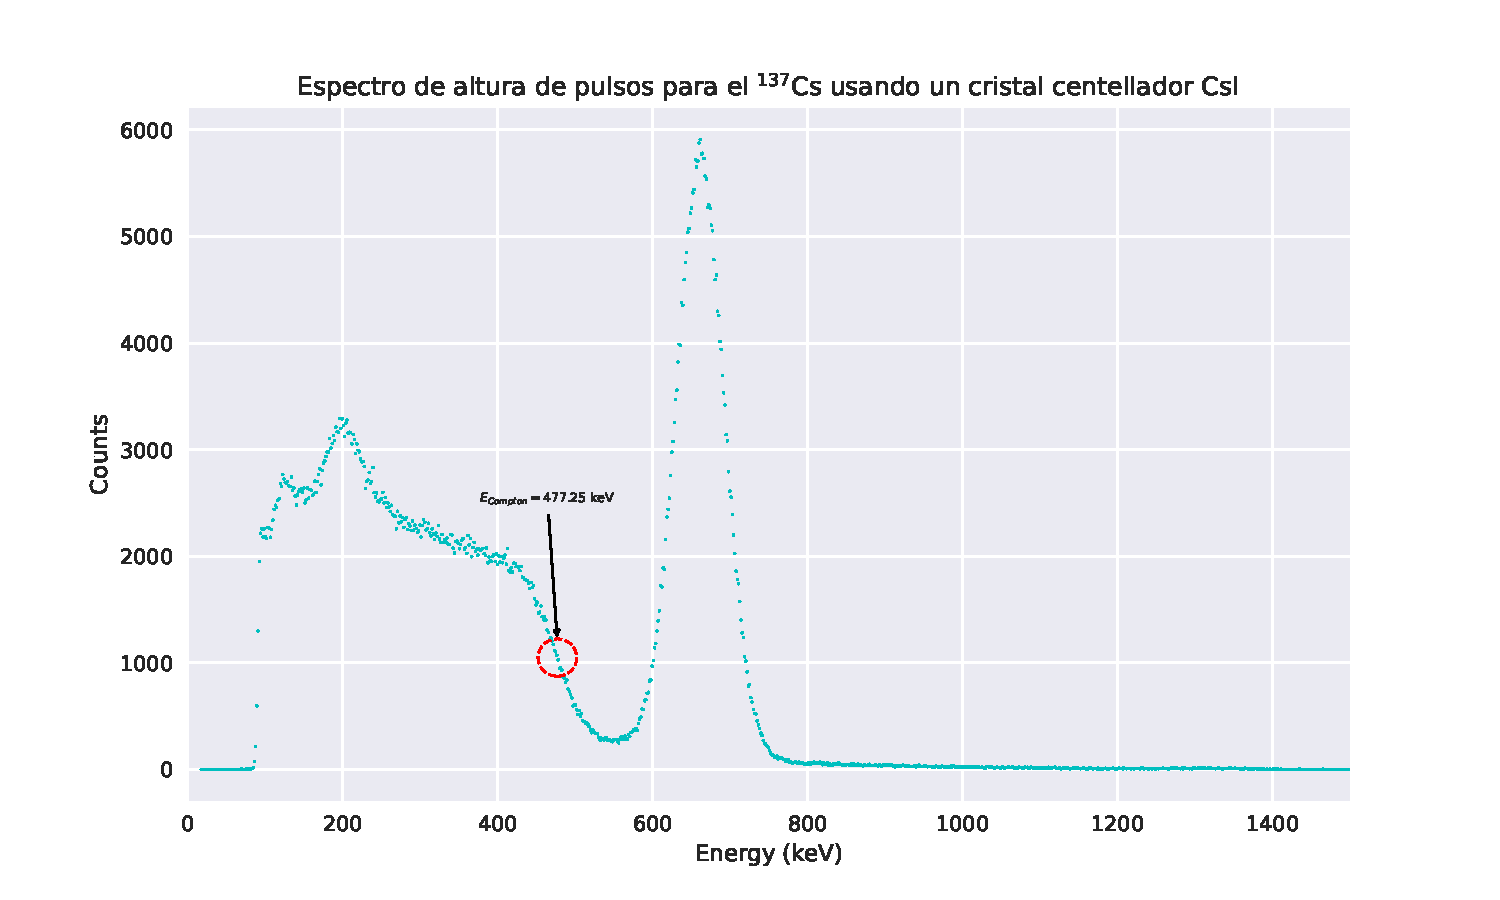
\includegraphics[scale=0.8, trim={1cm 0 1cm 0}, clip]{compton_edge_CsICs.pdf}
        \caption{Espectro de energía contra número de cuentas para la fuente de \ch{^{137} Cs} usando el centellador \ch{CsI (Tl)}. El valor del Hombro Compton está representado por el círculo.}
        \label{fig:comptonEdgeCsICs}
    \end{figure}

    \subsubsection*{Hombro Compton usando el centellador \ch{BGO (BiGeO)}}

    A partir de \cref{eq:comptonEnergy,eq:comptonEdge} tenemos que el Hombro Compton para cada una de las fuentes radioactivas es

    \begin{align*}
        E_{HC}^{\ch{^{60} Co}} &= \qty{963.42}{\keV},\\
        E_{HC}^{\ch{^{137} Cs}} &= \qty{477.33}{\keV}.
    \end{align*}

    Estos valores se encuentran representados aproximadamente mediante círculos en las \cref{fig:comptonEdgeBGOCo,fig:comptonEdgeBGOCs}.

    \begin{figure}[!htb]
        \centering
        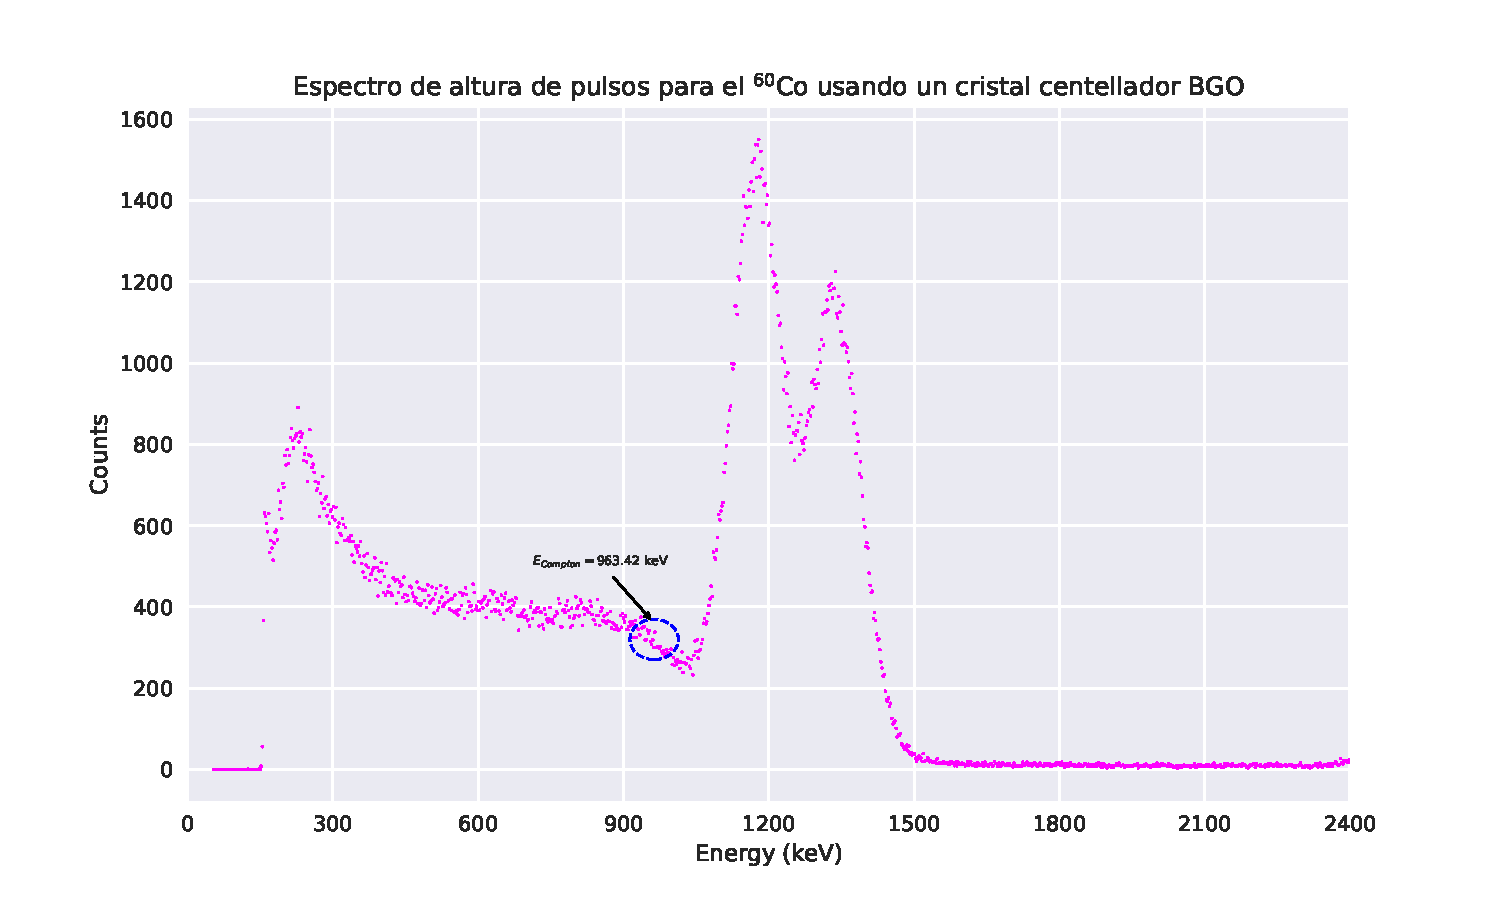
\includegraphics[trim={1cm 0 1cm 0}, clip, scale=0.8]{compton_edge_BGOCo.pdf}
        \caption{Espectro de energía contra número de cuentas para la fuente de \ch{^{60} Co} usando el centellador \ch{BGO (BiGeO)}. El valor del Hombro Compton está representado por el círculo.}
        \label{fig:comptonEdgeBGOCo}
    \end{figure}

    \begin{figure}[!htb]
        \centering
        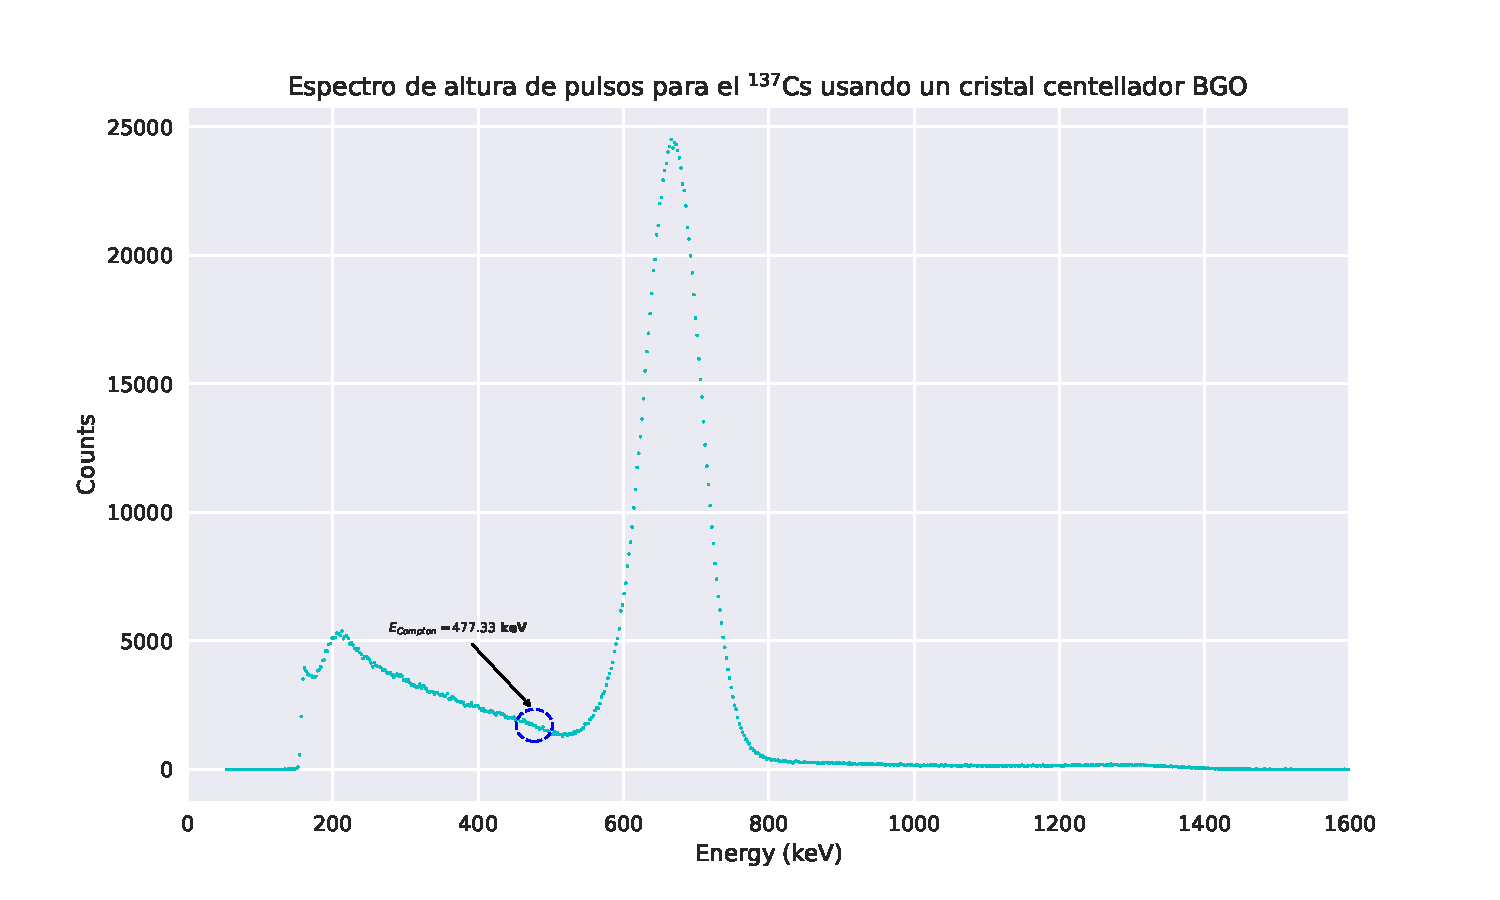
\includegraphics[trim={1cm 0 1cm 0}, clip, scale=0.8]{compton_edge_BGOCs.pdf}
        \caption{Espectro de energía contra número de cuentas para la fuente de \ch{^{137} Cs} usando el centellador \ch{BGO (BiGeO)}. El valor del Hombro Compton está representado por el círculo.}
        \label{fig:comptonEdgeBGOCs}
    \end{figure}

    \pagebreak
    \subsection*{Error relativo}

    Finalmente, calculamos el error relativo para los valores obtenidos del Hombro Compton y la energía del fotopico. Recordemos que el error relativo se calcula mediante

    \begin{equation}
        \epsilon_{r} = \dfrac{\Delta E}{E} \cdot \qty{100}{\percent},
    \end{equation}

    con \(\Delta E = \abs{E_{bd} - E_{m}}\), donde \(E_{bd}\) es el valor de la energía teórico y \(E_{m}\) el valor medido. 
    
    \pagebreak
    Por un lado, tenemos los resultados para los valores del Hombro Compton para cada uno de los centelladores, los cuales se encuentran en las \cref{tab:comptonErrorCsI,tab:comptonErrorBGO}.

    \begin{table}[!htb]
        \centering
        \begin{tblr}{
            colspec = {ccc},
            hlines,
            row{1} = {font = \bfseries}
        }
            Isótopo        & {Energía \\ (\si{\keV})} & $\varepsilon_{0}$          \\
            \ch{^{137} Cs} & \num{477.25}             & \qty{38.62}{\percent}       \\
            \ch{^{60} Co}1 & \num{963.42}                  & \qty{21.78}{\percent}       \\
            \ch{^{60} Co}2 & \num{1118.10}                  & \qty{19.17}{\percent}
        \end{tblr}
        \caption{Energía del Hombro Compton con su correspondiente error relativo usando el detector centellador \ch{CsI}.}
        \label{tab:comptonErrorCsI}
    \end{table}

    \begin{table}[htb]
        \centering
        \begin{tblr}{
            colspec = {ccc},
            hlines,
            row{1} = {font = \bfseries}
        }
            Isótopo        & {Energía \\ (\si{\keV})} & $\varepsilon_{0}$          \\
            \ch{^{137} Cs} & \num{477.33}             & \qty{38.62}{\percent}       \\
            \ch{^{60} Co}1 & \num{963.42}                  & \qty{21.78}{\percent}       \\
            \ch{^{60} Co}2 & \num{1118.10}                  & \qty{19.17}{\percent}
        \end{tblr}
        \caption{Energía del Hombro Compton con su correspondiente error relativo usando el detector centellador \ch{BGO (BiGeO)}.}
        \label{tab:comptonErrorBGO}
    \end{table}

    \pagebreak
    Por el otro, las energías de los fotopicos con sus respectivos errores relativos se encuentran en las \cref{tab:photopeakErrorCsI,tab:photopeakErrorBGO}.

    \begin{table}[htb]
        \centering
        \begin{tblr}{
            colspec = {ccc},
            hlines,
            row{1} = {font = \bfseries}
        }
            Isótopo        & {Energía \\ (\si{\keV})} & $\varepsilon_{0}$          \\
            \ch{^{137} Cs} & \num{661.10}             & \qty{0.064}{\percent}       \\
            \ch{^{60} Co}1 & \num{1166.67}                  & \qty{0.084}{\percent}       \\
            \ch{^{60} Co}2 & \num{1331.65}                  & \qty{0.56}{\percent}
        \end{tblr}
        \caption{Energía del fotopico con su correspondiente error relativo usando el detector centellador \ch{CsI}.}
        \label{tab:photopeakErrorCsI}
    \end{table}

    \begin{table}[htb]
        \centering
        \begin{tblr}{
            colspec = {ccc},
            hlines,
            row{1} = {font = \bfseries}
        }
            Isótopo        & {Energía \\ (\si{\keV})} & $\varepsilon_{0}$          \\
            \ch{^{137} Cs} & \num{666.77}             & \qty{0.773}{\percent}       \\
            \ch{^{60} Co}1 & \num{1178.78}                  & \qty{0.473}{\percent}       \\
            \ch{^{60} Co}2 & \num{1327.84}                  & \qty{0.349}{\percent}
        \end{tblr}
        \caption{Energía del fotopico con su correspondiente error relativo usando el detector centellador \ch{BGO (BiGeO)}.}
        \label{tab:photopeakErrorBGO}
    \end{table}


    \section*{Resultados y conclusiones}
    \kant[1]
    
    % \nocite{*} % Show all references    
    % Referencias
    \newpage
    \printbibliography
\end{document}